% Created 2022-09-29 Thu 16:44
% Intended LaTeX compiler: pdflatex
\documentclass[11pt]{article}
\usepackage[margin=1.5in]{geometry}
\usepackage[utf8]{inputenc}
\usepackage[T1]{fontenc}
\usepackage{graphicx}
\usepackage{longtable}
\usepackage{wrapfig}
\usepackage{rotating}
\usepackage[normalem]{ulem}
\usepackage{amsmath}
\usepackage{amssymb}
\usepackage{capt-of}
\usepackage{hyperref}
\usepackage{pdfpages}
\usepackage{makecell}
\usepackage[nottoc,numbib]{tocbibind}
\date{\today}
\title{\huge{Draft Report on Reproducibility and Data Policy -- Economica} \\ \vspace{5mm}\large(In progress -- may contain error.)}
%\subtitle{}

\begin{document}
\maketitle
\tableofcontents
\newpage

\section*{Executive Summary}
\begin{itemize}
\item In recent years, there have been a momentum on the part of economic journals towards adopting a data policy or upgrading the previous one. Currently, around 72\% of the top 100 journals, and 76 \% of the top 50 journals have some sort of data policy (for the ranking used and more details see Section \ref{landscape}).
\item The first version of a standard for code and data availability policies, prepared by a team of data editors of economic journals, was published in December 2022. \href{https://datacodestandard.org/}{\textit{DCAS}} seems to be the first important step toward homogenising the reproducibility and data policy of the economic journals and is expected to be endorsed by more and more journals in the coming months and years.
\item Endorsing DCAS and building a data repository ``community'' on Zenodo (or another comparable website) for a journal have near zero costs and seems to be a feasible option even for the smaller journals with lower budgets.
\item Enforcement, which consists of checking of the documentation and the data and code package as well as re-running the codes to ensure the internal consistency of the paper and the linked code/data (aka ``computational reproducibility'') is costly, but can be performed on different levels depending on the budget constraints. The recent experience of the \textit{Economic Inquiry} journal and \textit{Canadian Journal of Economics} offer useful insights for smaller journals to reconcile the increasingly demanding requirements of reproducibility with their lower levels of resources.
\end{itemize}

\newpage
\section*{Abbreviations}
\begin{itemize}
	\item \textbf{ICPSR}: Inter-University Consortium of Political and Social Research
	\item \textbf{DCAS}: Data and Code Availability Standard
	\item \textbf{RADE}: Restricted Access Data Environment
        \item \textbf{ARP}: Author Responsibility Policy (\cite{vlaeminck2015data})
        \item \textbf{DAP}: Data Availability Policy (\cite{vlaeminck2015data})
\end{itemize}

\newpage
\section*{Definitions}
\begin{itemize}
	\item \textbf{Research Data}: Contains both data and code (not only code of the main analysis but also codes for preparatory stages of final datasets).
	(\href{https://www.elsevier.com/authors/tools-and-resources/research-data}{Elsevier definition}),
	\item \textbf{Narrow Reproducibility}: obtaining consistent results using the same data and code
	as the original study. \cite{whited2023Costs}
	
	\item \textbf{Reproducibility}: “the ability of a researcher to duplicate the results of a prior study using
	the same materials and procedures as were used by the original investigator. So in an attempt to
	reproduce a published statistical analysis, a second researcher might use the same raw data to
	build the same analysis files and implement the same statistical analysis to determine whether
	they yield the same results.” \cite{bollen2015social}.\\
	Sub-categories according to \cite{dreber2023framework}
	\begin{itemize}
		\item \textbf{Computational Reproducibility}: To what extent results in original studies can be reproduced based on data and code posted or provided by the original authors. \cite{dreber2023framework}
		\item \textbf{Recreate Reproducibility}: To what extent results in original studies can be reproduced based on the information in the papers and access to the same raw data or data source, but without having access to the analysis code of the original study and/or the data set it was applied to.
		\item \textbf{Robustness Reproducibility}: To what extent results in original studies are robust to 		alternative plausible analytical decisions on the same data.
	\end{itemize}

        

	\item \textbf{Replicability}: “ the ability of a researcher to duplicate the results of a prior study if the
	same procedures are followed but new data are collected." \cite{bollen2015social}.
	\begin{itemize}
		\item Sometimes encompasses \textbf{generalisability}, extension of the scientific findings to other populations, contexts, and time frames. \cite{vilhuber2020reproducibility}
		\item \cite{hamermesh2007replication} calls this “scientific replication.” Robustness tests performed by researchers have aspects of self-replication,
	\end{itemize}
	\item \textbf{Grey literature}:	documents such as technical reports, working papers, and so on, that are typically not subject to peer-review but are of sufficient quality to be worth preserving and citing \cite{vilhuber2020reproducibility}. 
	
	
\end{itemize}


\newpage
\section{Introduction-- 2023: A Year of Replications and Retractions}

\qquad 2023 has been a year of increasing focus on credibility, in particular replicability, of economic research. \textit{Review of Economic Studies} retracted \cite{giuliano2014retracted}, the first retraction ever in its history, and \textit{American Economic Review} had its second retraction ever by retracting \cite{boissel2022dividend}. Less details were provided by \textit{REStud} regarding their retraction: `` While the original codes and data sets are no longer available, new analysis with a markedly similar data set does not support the original results.'' (\cite{restud2023retrac}). In the second case, authors of the falsifying comment which led to the retraction of the paper around one year after its publication, discover an error in the submitted code and, more crucially, show that main results of the published paper are sensitive to reasonable alternative specifications \cite{bach2023dividend}.\\

These retractions, along with revived reports around well-known works of Dan Ariely and other researchers have raised concerns, particularly among younger researchers in the profession, about credibility, and public perception of credibility, of economic research. Are we doing enough with respect to replication and reproduction of published articles?\\

One might also wonder how these events should be thought of in the light of the increasing investment of top economic journals in improving reproducibility and replicability standards in the recent years. A plausible explanation for the higher rate of retractions and withdrawals in economic (and finance) journals since early 2010s, in particular incidence of a handful of high level retractions in the past 1-2 years, is the increased transparency and more extensive and intensive enforcement of data availability standards. Greater transparency and data sharing requirements leading to less-costly scrutiny and more retractions should be deemed as a step forward for credibility of economic research.

The fact that availability of data and code is a first yet crucial step towards replicability of economic research has long been acknowledged. This should be what Ragnar Frisch had in mind when he wrote, in the editorial note of the first issue of \textit{Econometrica}:
\begin{quotation}
	In statistical and other numerical work presented in Econometrica the
	original raw data will, as a rule, be published, unless their volume is
	excessive. This is important in order to stimulate criticism, control,
	and further studies. \cite{frisch1933editor}
\end{quotation}
The same idea was recently echoed in the response of the editorial team of \textit{Journal of Finance} when they, in response to questions about their retraction of the award-winning paper \cite{rampini2020retracted}, stated that ``almost non-existence'' of retractions in economic and finance journals in the past has unlikely been due to absence of errors, but most probably caused by difficulty of replication [due to unavailability of the original data and code] as well as low incentives for replication efforts. They then explain how the recent introduction of mandatory data and code sharing by \textit{JFK} contributed to lower cost of replication by other authors and faster retraction of the original paper.\\


In this report, we are going to have a quick review on the \textit{status quo} of data policies in economic research, particularly with the aim of what can be done (and what cost) for journals which has not yet adopted a data policy (due to resource constraints). The organisation of this report is as follows. In Section \ref{hist} we will review the evolution of data policies in economic journals over the past two decades. In Section \ref{landscape} we offer a glimpse into the current landscape of data policy in the top-100 economic journals by looking at some descriptive statistics on types and components of data policy adopted by those journals. In Section \ref{conc} we aim to think about costs and benefits of upgrading data policy for journals with lower resources and conclude \footnote{I thank Joan Llull for his helpful comments, particularly with regard to different ``models'' currently in practice.}.

\newpage
\section{Data Policies in Economic Journals Since Early 2000s}
\label{hist}
\subsection{\textit{JPE} and Failure of the ``Replication Market''}
It goes without saying that replicability is necessary for credibility of findings in economics. The question is whether evolution and expansion of modern applied and empirical economic research since 1970s, has been accompanied and solidified by a proportionate number of replication exercises. Odds are that you answer in the negative to this question, as the majority of the handful of studies on replicability and reproducibility of economic papers give grounds for such a negative evaluation. \cite{dewald1986replication}, one of the earliest serious investigations of reproducibility of economic research, undertook the task of verifying reproducibility of all empirical articles published or accepted between 1980-1984 (or still under review in 1984) in the \textit{Journal of Money, Credit and Banking (JMCB)} (one of the pioneering journals with regard to data archiving and data policy). After contacting the authors twice (in more than 6 months), out of the total 154 article, they could obtain sufficiently complete data just for 8 of the articles. Their attempt in replicating 8 articles succeeded only for 5 of them\footnote{The authors mention their private correspondence with editor of another top journal confirming their belief that these sound like good estimates for other major journals, not peculiar to JMCB.}. More recently, \cite{chang2015economics} attempt to replicate 67 published articles in ``13 well-regarded economics journals using author-provided replication files that include both data and code.'' Excluding 8 papers which use confidential data or proprietary not-easily-accessible software, they succeeded in replicating no more than 29 (7 of these only with further assistance by authors), that is less than 49\% leading them to conclude that economic research is more often not replicable. Even as late as early July 2023 and despite all the progress that have been made in the past couple of years, \href{https://twitter.com/JoanLlull_econ/status/1675154240497483776}{Joan Lull}, the newly appointed data editor of the Econometric Society, stated that still around 60\% of data and code archives submitted would not reproduce the results (before verification).\\

Note that these dismal statistics pertain to the less ambitious concept of (computational) reproducibility: being able to successfully run a set of programs used by the authors of original papers on the original datasets, to obtain the same quantitative results as in the original papers. But reproducibility is hardly an end in itself; even with full computational reproducibility, the codes or data transformations might still contain errors, and even if they are error-free, they might simply be deemed as poor matches to the theoretical variables. Indeed, the criterion which is more closely-linked to credibility of findings in (economics) research is ``replicability''\footnote{\cite{maniadis2017replicate} develop a model of replication to find conditions for replications to succeed in safeguarding the credibility of economic research.} which deals with threats that are deeper and more complicated than those facing reproducibility, such as publication bias, specification searching and excessive occurrence of type-1 error (\cite{christensen2018transparency}). In the light of the evidence that errors in code and data are quite common (though in many cases not consequential for the results at stake), if a significant portion of publications in economics still fail to pass the looser requirements of reproducibility, one might wonder, how would they fare with respect to replicability and its implications for credibility of economic research.\\

Again, these concerns are not new: around half a century ago, \cite{feige1975consequences} published a comment in the \textit{Journal of Political Economy}, warning against common practice of economic journals in discounting (if not discarding) ``non-significant'' results and how this, on top of a lack of replicability exercises, can lead to ``data-grubbing'' and specification-hunting, thereby leading to a proliferation of Type-I error in the published articles. To avoid such an outcome, Feige argued, the journals need ``as a minimum standard'' to require authors to fully report their procedures and data, but also to filter articles more based on research design rather than final results (more similar to the way grants are awarded to research proposals). The editors of \textit{JPE}, while corroborating that these concerns are now widely acknowledged, denounced the proposed solution of Feige, on the basis its being both extremely costly and incapable of producing the right incentives, and propsed an alternative solution:

\begin{quotation}
  We believe that the true remedy is resort to the powerful force of competition. We believe that journals should be prepared to accept alternative statistical tests of a hypothesis, in which either the confirmation or the contradiction of the author's statistical tests is reported. For this task to be reasonably economical, any author should be willing to provide his underlying data to other scholars (at cost). Indeed, this behavior is a requirement for responsible scholarship.
\end{quotation}
They thus announced that they would add a new section to the \textit{JPE} called ``Confirmations and Contradictions'' which would publish brief yet comprehensive replication exercises (with no submission fees).\\

But, results of introducing this replication section in \textit{JPE} (and another journal, \textit{Journal of Consumer Research} (\cite{mayer1980economics}) was not encouraging. From 1976 to 1999, a total of 6 replication notes were published in the replication section of \textit{JPE} (5 of these belong to the period before 1987, of which only one was ``successful'' in replicating the original results,\cite{duvendack2015replications}). The section was quietly left to die thereafter.\\

Why such poor results? On the one hand replication is costly, in particular when the replicators do not have access to the original data and code. One the other hand, there is an incentive problem, replication is not generally regarded as a reward-worthy exercise. To quote \cite{dewald1986replication}:
\begin{quotation}
	Thomas Kuhn (1970) emphasized that replication-however valuable in the search for knowledge-does not fit within the
	``puzzle-solving'' paradigm which defines the reward structure in scientific research. Scientific and professional laurels are not awarded for replicating another scientist's findings.
	Further, a researcher undertaking a replication may be viewed as lacking imagination and creativity, or of being unable to allocate his time wisely among competing research projects. In addition, replications may be interpreted as reflecting a lack of trust in another scientist's integrity and ability, as a critique of the scientist's findings, or as a personal dispute between researchers. Finally, ambiguities and/or errors in the documentation of the original research may leave the researcher unable to distinguish between errors in the replication and in the original study.
\end{quotation}

In other words, replication exercises are public goods with significant positive externalities that at the same time incur large costs to individual researchers who are going to conduct them, without much benefits accruing to them as scholars. Facing such roadblocks, further progress seemed to be contingent upon changing the reward structure in a way that it becomes more conducive to replication exercises, as well as finding ways to cut the costs of replication and reproduction.\\

One way to achieve the last point could be to revisit the editorial policy suggested by Ragnar Frisch and quoted above: journals can make it mandatory for the authors to make their data and code publicly available. Before their papers get accepted, authors would have significant incentives to provide their data if it is a requirement for their paper getting published, and it will be much less costly for them to do so while conducting their research than for other researchers trying to redo all the similar steps on their own. This can hugely cut the costs of reproducing results of the original paper, which can make it much easier to further replicate those findings. Furthermore, the authors who make their data and code available, can make it easier for other researchers to build upon their results and methods, and get rewarded by getting cited more \footnote{\cite{renfro2004econometric} quotes Stephen Hall:''Another good example is the contrast between the Quandt disequilibrium models that
were around in the 70s and 80s and the Hamilton Markov switching. These two models are actually very
closely related but the Quandt models never caught on because essentially Dick Quandt never gave out the
software to implement them. Hamilton on the other hand gave out GAUSS code for everyone to do it and
so created a whole industry.''}. So data availability policy, appeared to be a naturally next step, and this was exactly the step that editors of \textit{Journal of Money, Credit and Banking (JMCB)} took in 1982.

\subsection{\textit{JMCB} and Data Availability Policy}
%\subsubsection{A bit of History: JMCB}
\textit{JMCB} put into force their  ``data availability policy'' in 1982; adopted an editorial policy of requesting from authors the programs and data used in their articles and making these programs and data available to other researchers on request. Results were encouraging; when as a sequel, they attempted to analyse the effect of this editorial policy on practical availability of data and code for reproduction, the submission rate of data and code for articles published before the announcement of the data policy was around 34\%, whereas for articles published after the announcement it rose to 74\%(\cite{dewald1986replication}). More importantly, a mandatory data and code policy seems to have led to less errors on the part of authors:

\begin{quotation}
Our findings suggest that the existence of a requirement that authors submit to the journal their programs and data along with each manuscript would significantly reduce the frequency and magnitude of errors. We found that the very process of authors compiling their programs and data for submission reveals to them ambiguities, errors, and oversights which otherwise would be undetected.
\end{quotation}

But at the same time, the experience of \textit{JMCB} showed some limitations of such a data policy. The first apparent problem was compliance. In the second phased of the project, when a team of researchers including an editor of the journal attempted to obtain data and code for replication, there were still 26\% of the authors who failed to submit their data and code \footnote{In one case, author of a paper which was submitted after the imposition of the new data policy but was still under review, failed to submit the data and code, saying that they have already lost or destroyed the data.}. The second issue was that, even among those who submitted their data and code, only 8 out of the 54 data sets were adequately documented. The most frequent problem was failure to precisely identify the source of the data. Replication issues were further exacerbated in many cases, by the mere fact that both the original data (think about \textit{Survey of Current Business} and software packages used to analyse data are both subject to regular revisions with no guarantee for backward compatibility. This would call for more careful citation and versioning practices to be adopted by economists\footnote{\cite{mccullough2006lessons} has a more extensive discussion of lessons of the JMCB experience.}.\\


William Dewald, editor of \textit{JMCB} from 1975-1983 played a pivotal role in adoption of a data policy and subsequent analysis of the results (\cite{dewald1986replication}). He was of course aware of the importance of permanence of data and code archives, so attempted to set up an on-premise archive using the good old floppy disks (\cite{mccullough2006lessons}). Unfortunately, subsequent events crashed his hopes of permanence, of not just the data he had archived but the very policy itself: after a change of the editorial team, not only the data policy was abandoned but also the files on floppy disks were discarded. This does not mean that the replication project pursued by Dewald was totally futile; in the same issue of \textit{AER} in which \cite{dewald1986replication} was published, editors of \textit{AER} announced a policy of requiring authors of the accepted articles to document their data and make it available upon request to any prospective replicator, though their policy fell short of requiring a mandatory data archive \cite{ashenfelter1986}. Few other journals such as \textit{Journal of International Economics} and \textit{Journal of Human Resources} followed suit. Furthermore, after Dewald was appointed director of research at the Federal Reserve Board of St. Louise in 1992, he again implemented a data/code archive for the \textit{Review} and started to conduct an in-house replication verification of each article prior to publication. \textit{Federal Reserve Bank of St. Louis Review} switched to a web-based archiving system in 1995 (\cite{anderson2008role}).

\subsection{Progress Since Early 2000s}
\subsubsection{Data and Code Availability Policy: \textit{AEA} Takes the Lead}
The \textit{JMCB} itself started again to implement a mandatory data and code availability policy in 1996, with online archiving now available thanks to the growth of world wide web. More importantly, its experiment, with accompanied successes and failures well reported and analysed by \cite{dewald1986replication}, could have been an instructive case to be followed up by more robust and better designed policies on the part of economic journals. However, while \textit{Federal Reserve Bank of St. Louis Review} drew upon \textit{JMCB}'s experiment to adopt a stronger data policy, apparently, these lessons were slow to diffuse and not sufficiently paid attention to on a more general scale. In their \textit{AER} paper, \cite{mccullough2003verifying}, after demonstrating what can go wrong with nonlinear solvers of some of the most widely used pieces of statistical software and warning against the naiveté displayed by even some of the top econometricians with regard to the software, put the issue of ``software-dependency'' of some of the published results in applied economics in the more broader context of replicability and reproducibility. They first complain about an utter lack of data policy in some of the top journals:
\begin{quotation}
 What is difficult to believe is that 17 years
after Dewald et al. (1986), most economics
journals have no such policy, e.g., Journal of
Political Economy, Review of Economics and
Statistics, Journal of Financial Economics,
Econometrica, Quarterly Journal of Economics, and others. One cannot help but wonder
why these journals do not have replication policies. Even in the qualitative discipline of history, authors are expected to make available
their data...
\end{quotation}

Moreover, they criticise \textit{AER} and few other journals which had a mere replication policy (APR), for inefficiency of their policy. While the \textit{AER} had implemented a policy of ``Details of computations sufficient to permit
replication must be provided,'' \cite{mccullough2003verifying} reported results of their own investigation of applied economic articles in the June 1999 issue of this journal to show that about half of the authors would not honour this policy. They proposed that the economic journals had better implement a mandatory data and code availability policy stored in an archive managed by the journal itself, something that has become possible and easily affordable thanks to the expansion of the internet. They stated that at the time of their writing, only 3 journals had such a policy in place: \textit{Federal Reserve Bank of St. Louis Review}, \textit{JMCB} and \textit{Macroeconomic Dynamics}, and a fourth journal, \textit{Journal of Applied Econometrics} that had a similar policy but only for data (excluding the code).\\

In response to \cite{mccullough2003verifying} the \textit{American Economic Association (AEA)} announced
its new (mandatory) ‘data availability policy’ in 2003, implemented it in 2004, and extended it to the new domain-specific
journals in 2009–2012. The \textit{JPE} announced its
policy in 2004 and implemented it in 2005 and other top journals followed in the footprint of \textit{AEA} (\cite{vilhuber2020reproducibility}). \textit{AEA} has since spearheaded a significant progress in data and code policy of the economic journals. While a data and code policy sounds, \textit{prima facie} simple and straightforward to implement, there are intricacies to deal with. Apart from the more problematic issue of confidential and proprietary data (which are themselves different from the so-called ``secret data''), there are ambiguities and misunderstanding about some of the publicly accessible data sets and how one should properly cite and archive them in order to make reproduction of the results, less daunting. For example, \cite{vilhuber2020reproducibility} explains:
\begin{quotation}
Some widely used data sets are accessible by any researcher, but the license they are subject to prevents their
redistribution and thus their inclusion as part of data deposits. This includes nonconfidential data sets from the
Health and Retirement Study (HRS) and the Panel Study of Income Dynamics (PSID) at the University of
Michigan and data provided by IPUMS at the Minnesota Population Center. The typical user will create a custom extract of the PSID and IPUMS databases through a data query system, not download specific data sets. Thus, each extract is essentially unique. Yet that same extract cannot be redistributed, or deposited at a journal or any other archive. In 2018, the PSID, in collaboration with ICPSR, has addressed this issue with the PSID Repository, which allows researchers to deposit their custom extracts in full compliance with the PSID Conditions of Use. \footnote{For IPUMS, extracts from population samples (e.g., the 5\% sample of the U.S. population census) rather
than full population censuses (the 100\% file) can be provided to journals for the purpose of replication. (end-note 19 of \cite{vilhuber2020reproducibility})} 
\end{quotation}

\cite{vilhuber2020reproducibility}, \cite{vilhuber2023Reinforcing} and \cite{vilhuber2023reproducibility} provide more details on the progress made and in particular, on current best practices.

\subsubsection{Data Archiving}
We already mentioned how the \textit{JMCB} experience showcased the importance of a data archive for journals seeking a sound data policy. One of the earliest attempts was by \textit{JMCB}'s Dewald  trying to build a floppy-disk based data archive; an attempt which failed but was replicated by Dewald in his capacity as research director of the Federal Reserve Board of St. Louise. This last attempt later on transcended to a web-based archive starting 1995. In parallel and in-between the two attempts by Dewald, \textit{the Journal of Applied Econometrics} set up a data archive in 1988. However, these used to be exceptions rather than norm. Even by as late as early 2000s, most journals, including those few which had set up some kind of replication policy, used to discard having a proper archive. Was it because of the costs? Probably not, because according to \cite{anderson1994replication} even when National Science Foundation offered journals a free archive, editors refused to make use of it. The reluctance of economic journals to adopt and enforce a data and code archive policy for such a long time, is still a bit puzzling. Whatever the reason, it took about 2 decades for the most prestigious journals in the field of economics, to move away from that equilibrium.\\

It took several years for \textit{QJE} and other top journals to adopt the \textit{AER}'s policy. Even then, most of the journals preferred to use their own websites to archive the data and code. However, during the past several years, an increasing number of economic journals have started to set up their archives on proper data repositories, such as ICPSR, Harvard Dataverse and Zenodo, which seem to offer not just probably more longevity, but also a unique digital identifier to data and code, making citation and reproduction much less troublesome(\cite{vilhuber2020reproducibility}. \cite{currier2021safeguarding} use content analysis to provide a more detailed review of current status and enforcement of data preservation policies in economic journals.

\subsubsection{Documentation}
As mentioned above, \cite{dewald1986replication} report lack of proper documentation to be a big issue for reproduction exercises. With data sets having become larger and larger over time, and codes and programs commensurately having got increasingly complicated, navigating the data and code of a typical article wanting proper documentation has become evermore daunting. This was confirmed by later attempts at reproduction, e.g., by \cite{mccullough2003verifying} when they set to investigate the degree of compliance of authors who submit to \textit{AER} with the announced (ARP) replication policy. They recount 
\begin{quotation}
A third author, after
several months and numerous requests, finally
supplied us with six diskettes containing over
400 files—and no README file. Reminiscent of the attorney who responds to a subpoena with
truckloads of documents, we count this author
as completely noncompliant.
\end{quotation}

Similarly, in their attempt to replicate the papers in the \textit{JMCB} archive, \cite{mccullough2006lessons} report various cases where lack of documentation of data or code makes it virtually impossible to reproduce the research, e.g.,
\begin{quotation}
One author provides no readme file and two data files with no column
headers: we are supposed to guess the names of the variables!
\end{quotation}
Therefore they recommended journals to require authors to provide ReadMe files for the whole data and code files, documentation for the code and a code-book for the data.\\

Yet the most advanced and recent progress in this aspect is the recommendations put forth by authors of the DCAS standard, a joint effort of a small team of leading data editors of the economic journals which we will talk about more below. They have some recommendations for data/code sharing including documentation, which we have reproduced in the Appendix section \ref{dcas_table}, as well as a template ReadMe file which we have included in Appendix section \ref{dcas_readme}.

\subsubsection{Data Availability Statement}
Last but not least, inclusion of a data availability statement gradually proved to be a useful component for reproduction exercises. \cite{mccullough2006lessons} complain that for some of papers they were attempting to reproduce, there were no datasets but also no indication or statement that the data is confidential though they were sure some of those paper had used confidential data. More importantly and contemporaneously, data availability statements are nowadays supposed to provide sufficiently detailed guidance for other researchers who seek access to the original data, including any limitations and the expected monetary and time cost of data access \cite{koren2022dcas}. 

\subsubsection{DCAS: Data and Code Availability Standard}
A promising and welcome development towards a more comprehensive, thoughtfully designed and agreed-upon data policy standard for publications in economics (and social science at large) emerged in mid-December 2022, by launching of the first version of \href{https://datacodestandard.org/}{\textit{DCAS}}, the ``Data and Code Availability Standard''\footnote{https://datacodestandard.org/}.
This is the result of a joint effort by data editors of economic journals Miklós Koren (\textit{Review of Economic Studies}), Marie Connolly (\textit{Canadian Journal of Economics}), Joan Llull (\textit{Economic Journal} and \textit{Econometrics Journal}; since July 2023 \textit{The Econometric Society}) and Lars Vilhuber (\textit{AEA}) to come up with a well-designed standard for sharing research data and code.

As of today (12th of August of 2023), DCAS is endorsed by
\begin{itemize}
\item AEA Journals
\item Canadian Journal of Economics
\item Econometric Society Journals
\item Royal Economic Society Journals
\item Economic Inquiry
\item Review of Economic Studies
\end{itemize}

\subsection{Compliance: Data Policy Verification as an Editorial Function}
We already discussed how, despite the positive effects of introducing an author responsibility type of policy (as with Ear's initial replication policy) or even a stronger mandatory archive policy,
compliance remains far from perfect. There are disincentives for economists to spend time on ensuring replication, compiling the code and data to get them readily available for independent researchers to conduct reproduction exercises, thoughtfully documenting everything, conceivably conducting more checks before send them out to journals are all time consuming (see \cite{feigenbaum1993market} for a more detailed discussion of why economists might dislike reproducible research, for good reasons!)

\cite{dewald1986replication} point out one of the limitations of the first policy of \textit{JMCB}:
\begin{quotation}
enforcing matters, even for the 65 authors whose manuscript were under review, only 49 responded for a request for submitting of Data and Code while they had accepted it as mandatory, with a mean response time of 130 days; and from this 49, a further 18 did not submit the codes and data, in one case based on the reason that they had already lost or destroyed the data (before a decision has been made on their manuscript.)
\end{quotation}

Even after upgrading of the \textit{JMCB} data policy to mandatory data archiving, \cite{mccullough2006lessons} conclude their paper aimed at evaluating results of this policy by complaining that they could at the end just reproduce 22\% of the candidate papers that were submitted under the new policy. They conclude that more checks should be done on the part of journals.\\

It is not surprising then that gradually, pioneering journals moved towards introducing a formal verification process as part of the editorship functions. Today about a dozen of top journals have formal enforcement processes, and this with varying degrees, which may include editorial monitoring of the contents of the supplementary materials, reexecution of
computer code (verification of computational reproducibility), assessing the feasibility of data access reproduction is an integral part of a data editor's tasks, and improved archiving of data \cite{vilhuber2020reproducibility}. However, having a data editor seem to be one of the more expensive components of data policy, in particular for the smaller journals.\\

In the next section we will have a closer look at the current state of data policies in a larger sample of journals.



\newpage
\section{A Glimpse into the Current Landscape of Data Policy in Economic Journals}
\label{landscape}
In this section we will have a quick look into the \textit{status quo} of research data policies of economic journals. To this end, we summarise the data policy of the top 100 journals in Economics, based on surveying of the relevant sections on their websites, such as ``authors' guideline'' or ``data policy'' (In many cases journals have two websites, one of the publisher and another of their own) \footnote{A caveat is, in some cases the wording is more or less vague, and journals with very similar wording of the same component of data policy, might significantly differ in how they implement that part.}.\\

While there is no universally accepted way to rank and choose journals, in this section, we follow the most recent publication on ranking of economic journals (\cite{ham2021new}). The goal is to have a criterion for cutting the large number of journals that can be included in the statistical analysis, to get a sense of how the data policy ``moments'' change with the percentile (top-5, top-25, etc.), and what the current situation is for journals which are more or less on the same ``tier'' as \textit{Economica}. We chose 100 to limit the size of the sample, because economica seems to be ranked between 40-70 in a couple of more widely used new rankings (it ranks 45 according to the aforesaid ranking). Note that this set of journals do not contain survey-type journals such as \textit{JEP} or \textit{JEL}, nor the finance journals. 

\subsection{Summary of the \textit{Status Quo} of Data Policies}
We investigate the data policy of journals on six dimensions:
\begin{enumerate}
\item Is there any kind of data and replication policy? And what kind?
\item Is there a mandatory data/code sharing policy?
\item Does it also contain mandatory documentation?
\item Is data availability statement mandatory?
\item What kind of repository do they employ (if any)?
\item Does the editors perform any verification to enforce the policies?
\end{enumerate}

Table \ref{tab:summary} shows a summary of the results. Out of the top 100 journals, 73\% have some kind of data policy, 13\% of them have data editors, 43\% require authors to submit a data availability statement, 59\% require authors to share data and code, and 41\% explicitly require authors to have documentation of data/code included. Among the top 50 journals, around 80\% have some kind of data policy and 70\% require authors of accepted papers to share their data and code. In the following subsections, we dig into the details of each component.

\begin{table}[htbp]
   \centering
   \caption{{Summary of Data Policy in the Top 100 Econ 
     Journals \\ (\%)}}
   \vspace{7mm}
   {\label{tab:summary}
  \begin{tabular}[c]{l|c|c|c|c|c}
   & \thead{Any Data\\ Policy} & \thead{Data Editor}  & \thead{Data Availability\\ Statement} & \thead{Data \& Program\\ Sharing} & \thead{Documentation\\ (ReadMe)}\\
    \hline \hline
    Top 5 (\%) & 100 & 60 &80 &100 &100 \\
    %\hline
    Top 25 (\%) & 88& 40 &56 &84 &76 \\
    %\hline
    Top 50 (\%) & 76 & 24 &42 &68 &60 \\
    %\hline
    Top 75 (\%) &74.7& 17.3 &41.3 &64 &49.3 \\
    %\hline
    Top 100 (\%) &72& 13 &42 &58 & 41 \\
    \hline \hline
%\vspace{4mm}
  \end{tabular}
   }
\end{table}



\subsection{Types of Data Policies}
Different types of data policies currently used by journals appear to fall into 4 main categories: DCAS, AER policy, own data policies specific to the journal, and data policies of the publisher.\\

Table \ref{tab:avail} shows the distribution of different types of data policies. As of 12 August of 2023, three out of the type 5 journals have endorsed DCAS, including \textit{AER} and all journals of the AEA family. The remaining two, \textit{QJE}\footnote{QJE declares its data policy to be the AER data availability policy. However, it recommends the ReadMe Template of the ``Social Science Data Editors'' website.} and \textit{JPE} are still following the previous version of \textit{AER} data policy. Over the whole 100 top journals, those that have adopted DCAS are:
\begin{itemize}
\item AEA Journals
\item Canadian Journal of Economics
\item Econometric Society Journals
\item Royal Economic Society Journals
\item Economic Inquiry
\item Review of Economic Studies
\end{itemize}

For now there seems to be no journal out of top-100 that have adopted DCAS. There are also more ambiguous cases. For example, \textit{Journal of European Economic Association} recommends DCAS and states on part of its website that their policy is ``compatible with DCAS,'' but it is not clear whether they really require it or not.\\

Note that some journals seem to have adopted a data policy as suggested by their publishers. In particular Elsevier, and Springer seems to have data policies of different orders. For example, Most of the economic journals published by Springer, who do not follow DCAS or older AER nor they have their own data availability policy, seem to follow Springer's Type 3 Research Data Policy which mandates provision of a data availability statement but only encourages sharing of data and code (e.g., Journal of Economic Growth, Journal of Risk and Uncertainty). Occasionally They follow Type 1 or Type 2 (e.g., Public Choice, and Review of World Economy). However, Springer has planned to rule out Type 1 and 2 from Summer 2023. Visit the appendix \ref{springer} For more details on legacy and new Springer data policies\\

Regarding Elsevier, most of our journals with an Elsevier data policy, require sharing of data and code after an article has got accepted, before publication (e.g., Journal of Public Economics and International Journal of Industrial Organisation). What was not clear from the webpages, was that whether it is really enforced or not (a cursorily search for a couple of instances did not lead to any particular data archive.) Few of them require authors to submit a data availability statement. More importantly, it seems that Elsevier is trying to ``push'' Mendeley as the data archive of choice for journals that want to do it, though there are few cases, such as \textit{Explorations in Economic History} in which journals have prioritised Open-ICPSR or other trusted repositories. All in all, it seems like in the majority of cases where there is no strong commitment of journal editors to DCAS or some particular data policy, the end result might be a combination of publishers' practices and editorial team preferences (these all should be taken with a grain of salt as we do not have strong evidence for them!)\\



\begin{table}[htbp]
   \centering
   \caption{{Types of Data Availability Policies in the Top 100 Econ 
     Journals \\ (\%)}}
   \vspace{7mm}
   {\label{tab:avail}
  \begin{tabular}[c]{l|c|c|c|c}
   & \thead{DCAS} & \thead{AER}  & \thead{Own Policy} & \thead{Publisher's}\\
    \hline \hline
     Top 5 (\%) & 60 & 40 &0 &0 \\
    %\hline
    Top 25 (\%) & 44& 16  &20 &12 \\
    %\hline
    Top 50 (\%) & 24 & 10  &28 &18 \\
    %\hline
    Top 75 (\%) &18.7& 6.7 &25.3 &28 \\
    %\hline
    Top 100 (\%) &14& 5 &29 & 29 \\
    \hline \hline
%\vspace{4mm}
  \end{tabular}
   }
\end{table}


\subsection{Data Editors}
Few journals have specific data editors at the moment. These include Lars Vilhuber for AEA journals, Marie Connolly for the \textit{Canadian Journal of Economics}, Joan Llull for the \textit{Econometrics Society} journals, Miklos Koren for the \textit{REStud}, and Florian Oswald for the \textit{Royal Economic Society} journals.\\

However, there are other cases which are a bit fuzzy. For example, there are indications in the website of \textit{Review of Economic Dynamics}, that Christian Zimmermann performs some of the functions which are usually part of data editors' job (archiving and some sort of quick checking?) Also, the journal of \textit{Economic Inquiry} do not name any data editor on their website, but state that ``a member of the editorial board will review the data archive to ensure that it meets the journal requirements.''\\

\subsection{Data and Program Sharing Requirements and Archiving}
Most journals that have mandatory data and code sharing policy, manage an archive of the linked data and code of their published articles, either on their own website or on a public repository. In few cases, journals have announced a mandatory data and code sharing while it seems like they do not have a specific archive. Their guides usually recommends or suggests that authors put their data and code on a public repository (or one from the lists supported by the publisher) and include a link, e.g., in their data availability statement.\\


One ambiguity regarding the mandatory sharing of data and code that we alluded to above is for those journals that adopt Elsevier's data policy and announce a mandatory data sharing policy, though it is not clear whether they enforce this or not. We also mentioned that it seems like Elsevier is pushing for Mendeley Data to become the main archive for journals published by them.\\


\begin{table}[htbp]
   \centering
   \caption{{Data Repository in the Top 100 Econ 
     Journals \\ (\%)}}
   \vspace{7mm}
   {\label{tab:repo}
  \begin{tabular}[c]{l|c|c|c|c|c}
   & \thead{ICPSR,\\ Zenodo or \\ Harvard Dataverse} & \thead{``Public Repositories''}  & \thead{Journal's\\ Website} & \thead{Mendeley} & \thead{Publisher's\\ List}\\
    \hline \hline
    Top 5 (\%) & 100 & 0 & 0 & 0 & 0 \\
    %\hline
    Top 25 (\%) & 52& 4 & 16 & 4 & 20 \\
    %\hline
    Top 50 (\%) & 38 & 10 & 12 & 12 & 30 \\
    %\hline
    Top 75 (\%) & 32 & 6.7 &12 & 9.3 & 36 \\
    %\hline
    Top 100 (\%) & 26 & 13 & 9 & 7 & 33 \\
    \hline \hline
%\vspace{4mm}
  \end{tabular}
   }
\end{table}

All in all there are some journals which archive they data on one of the ``trusted repositories'' (see \cite{connolly2023journal} for an update and detailed guide on the importance and choice of repositories.) Overall, of the top-100 journals, 5 use a Harvard Dataverse Repository, 8 use the Open-ICPSR (including 5 AEA journals) and 6 use Zenodo. \textit{Journal of Applied Econometrics} uses ZBW Journal Data and \textit{Canadian Journal of Economics} uses the Dataverse on Borealis. 8 journals use their own websites to archive data. See Table \ref{tab:repo} for more details of the distribution of the repository policies. Note that the columns are not necessarily mutually exclusive. E.g., Mendeley is also an instance of Publisher's List, but we put it in a separate column to single out cases where Mendeley is the only archive named/used by the journal. Also in some cases, there are combinations like ``Mendeley or a comparable public repository,'' etc.\\





\newpage
\section{Conclusion: Trade-offs for Smaller Journals}
\label{conc}
%\label{small}
Replicability of research findings in a discipline is a key to its credibility. But replicability is very costly to verify, and its verification often goes beyond findings of a single manuscript and ``involves agreements and disagreements among research papers which form a body of literature'' around some given question or result (\cite{vilhuber2023reproducibility}). What is less costly to verify and, in turn, a key prerequisite for verifying replicability, is the limited notion of reproducibility which is something that can be verified and enforced by the journals (with varying degrees of intensity depending on the budget) for any single manuscript. \\

Despite being a more modest goal, reproducibility, even in the narrower sense of computational reproducibility, is still a costly good to produce. It is costly for the authors because it takes time to compile the code and to document the data up to the required standards. %What could also imagine that authors might put more time and resources in verifying their codes if they know that it would become publicly and permanently available and linked to the published paper. 
These costs are conceivably increasing over time as both processing of data and programs become more and more complicated. There are also additional costs if the underlying data is confidential, or when the analysis is high-dimensional. Finally, there might be some equity concerns as reproducibility requirements are particularly burdensome for authors who cannot afford research assistance. But reproducibility policies, or even the more limited mandatory data and code sharing policies have benefits. They not only benefit the whole discipline, but also the individual authors by decreasing the likelihood of error on their part. To quote \cite{dewald1986replication}:
\begin{quotation}
	Our findings suggest that the existence
	of a requirement that authors submit to the
	journal their programs and data along with
	each manuscript would significantly reduce
	the frequency and magnitude of errors. We
	found that the very process of authors compiling their programs and data for submission reveals to them ambiguities, errors,
	and oversights which otherwise would be undetected.\\
\end{quotation}

Reproducibility checks are also costly for journals. Checking the documentations to see whether they conform to the required standards, verifying that the data availability statement makes sense and can direct other researchers towards obtaining the data, and last but not least, re-running the computer programs to see whether they can produce the same graphs and tables as in the original paper are all costly to conduct. This pecuniary costs can be substantial if a journal is going to conduct checks thoroughly and systematically, as it involves hiring data editors and well-trained research assistants, while many academic journals run on tight budgets \footnote{While the pecuniary costs can differ substantially between journals, depending on what data policy they have and how thoroughly they are going to check the submitted packages, Lars Vilhuber gives an estimate of the total reproducibility budget to be around twice as much as an editor gets paid (\cite{crress2022session1})}.\\

Such costs can be particularly concerning for smaller journals, not only the pecuniary costs but also side damages such as a possible cut to submissions if the prospective submitting authors consider the data policy as burdensome. However, there are still low-cost steps that can be adopted by journals to contribute to the collective movement towards higher reproducibility. It was previously suggested that adopting the DCAS and setting up a repository on Zenodo have almost no cost. Moreover, side damages should probably not be a big concern based on the recent report of the editor of \textit{Economic Inquiry} who that drop in the submission rate was not high (it was around 15\% in the subsequent year after introducing the policy and extra checks.) Even this low cost might mean revert to zero as more and more journals move towards adopting data policies \footnote{See \cite{whited2023Costs}, \cite{chang2015economics} and \cite{anderson2008role} for more detailed discussion of costs and benefits of data and replication policies.}. \\


To wrap up, adopting and enforcing a data policy have clear benefits, while pecuniary costs can range from a minimum of around zero to a maximum of about twice the payment of an editor. The near zero cost policy could be to just endorse the DCAS and build a community on Zenodo or another similar trusted repository, and require authors to submit their data and code packages to the linked depository without any systematic checking and verification for the moment. The intermediate option is to check the data and documentation without rerunning all the code. The more complete solution involves a full checking which might be too costly for a small journal with lower resources. Journal of \textit{Economic Inquiry} and the \textit{Canadian Journal of Economics} offer useful insights into how to conduct a less demanding and basic, yet financially feasible, level of verification. For example, \textit{Canadian Journal of Economics} checks that packages are complete and include all the documentation and the ReadMe file passes the minimum requirements, but does not run reproducibility checks \footnote{There are other options such as outsourcing to CASCAD which might have benefits for smaller journals.}.




\newpage
\appendix
\section{DCAS: Data and Code Availability Standard}
\subsection{DCAS Table}
\label{dcas_table}
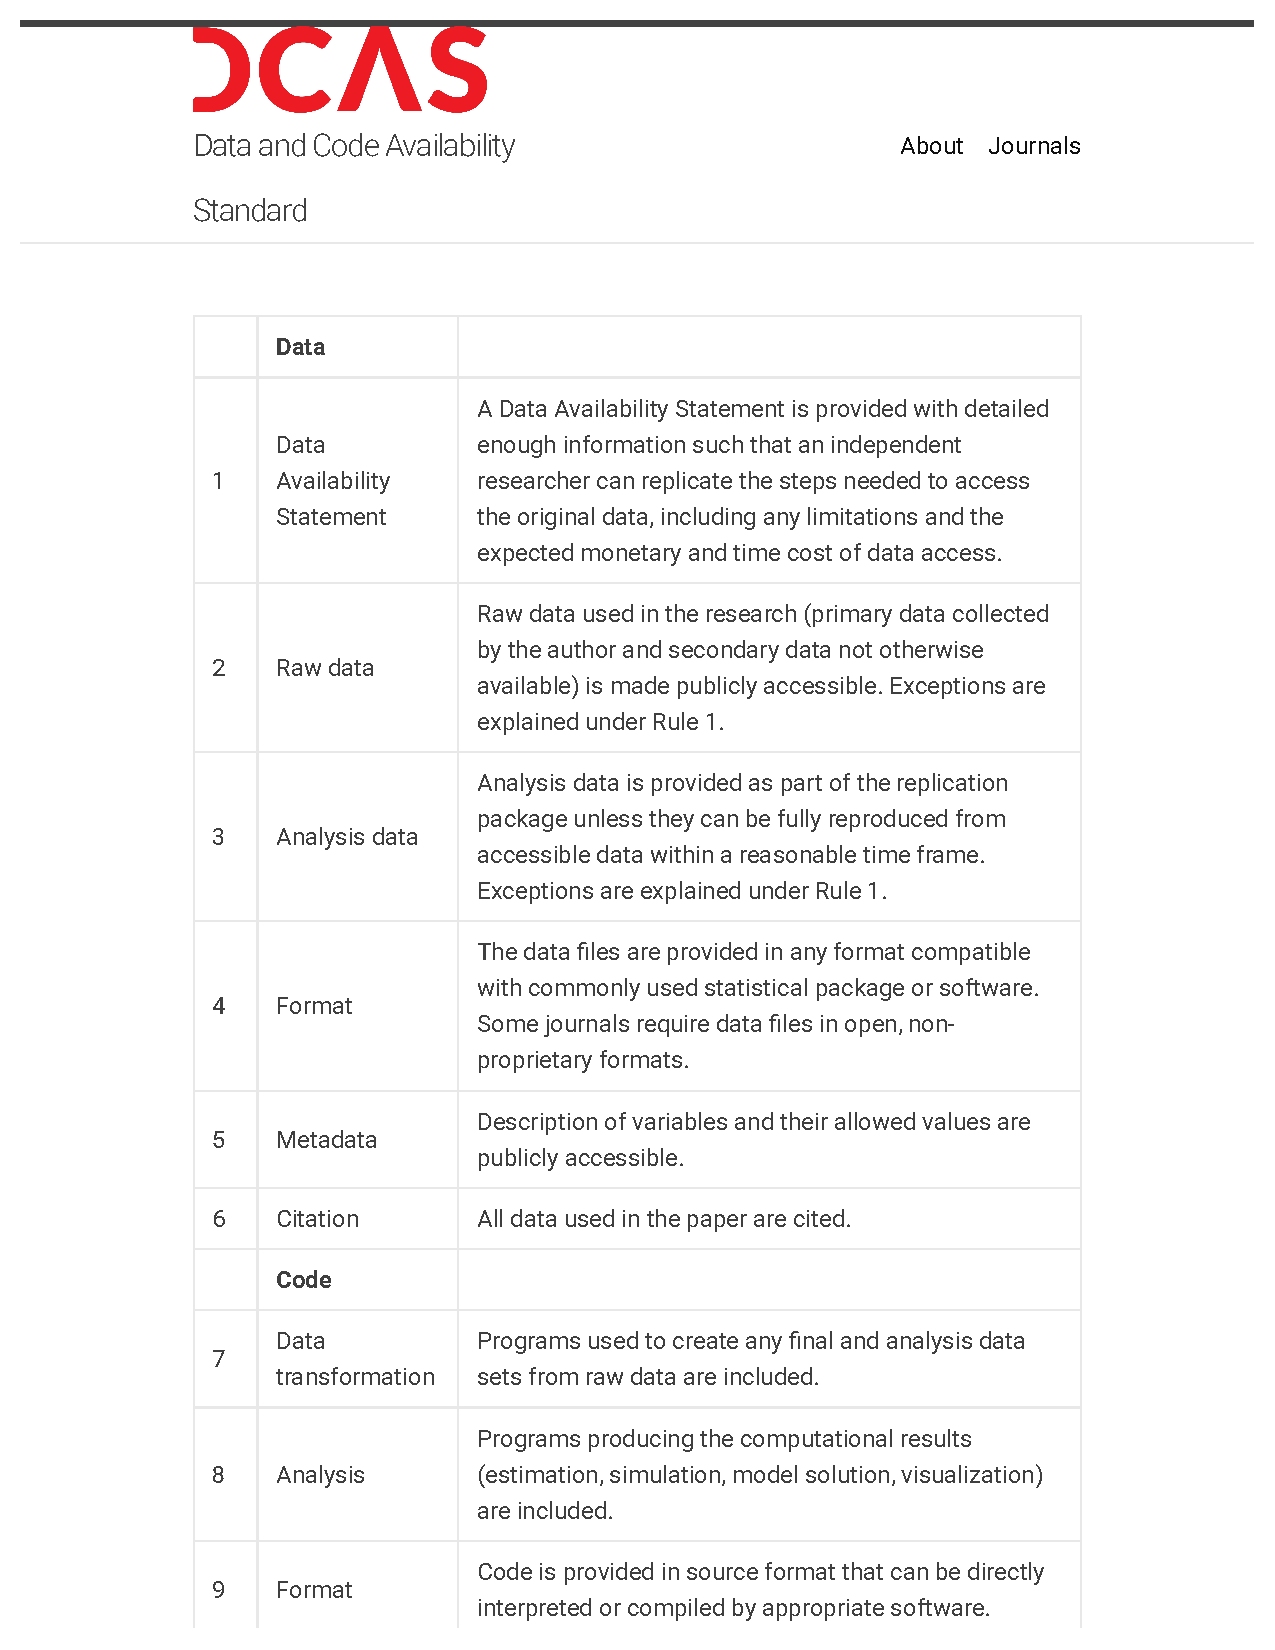
\includepdf[pages=-, scale = .8]{dcas_table.pdf}

   

\subsection{DCAS Template for the README File}
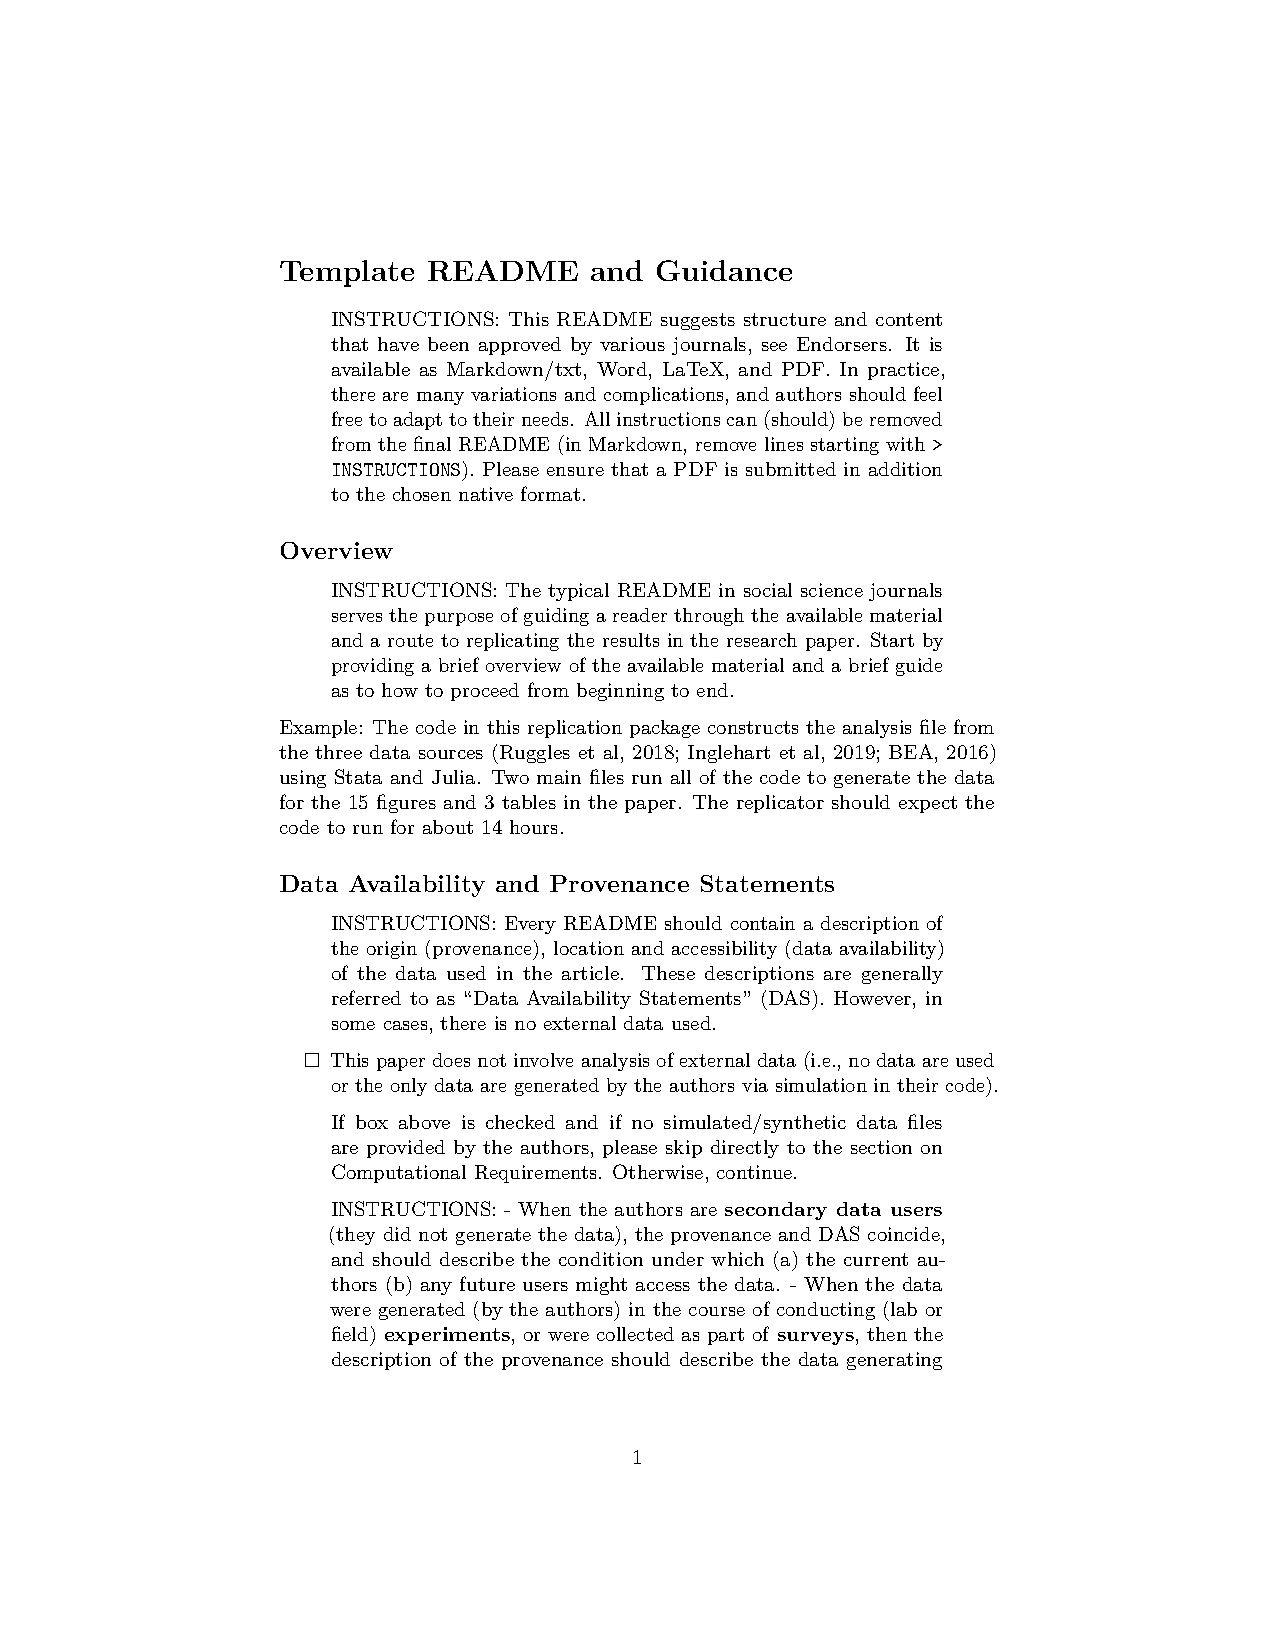
\includepdf[pages=-,pagecommand={\subsubsection*{DCAS ReadMe Template}\label{dcas_readme}}, scale=.8]{README.pdf}


\section{AER}
\subsection{AER Data and Code Availability}
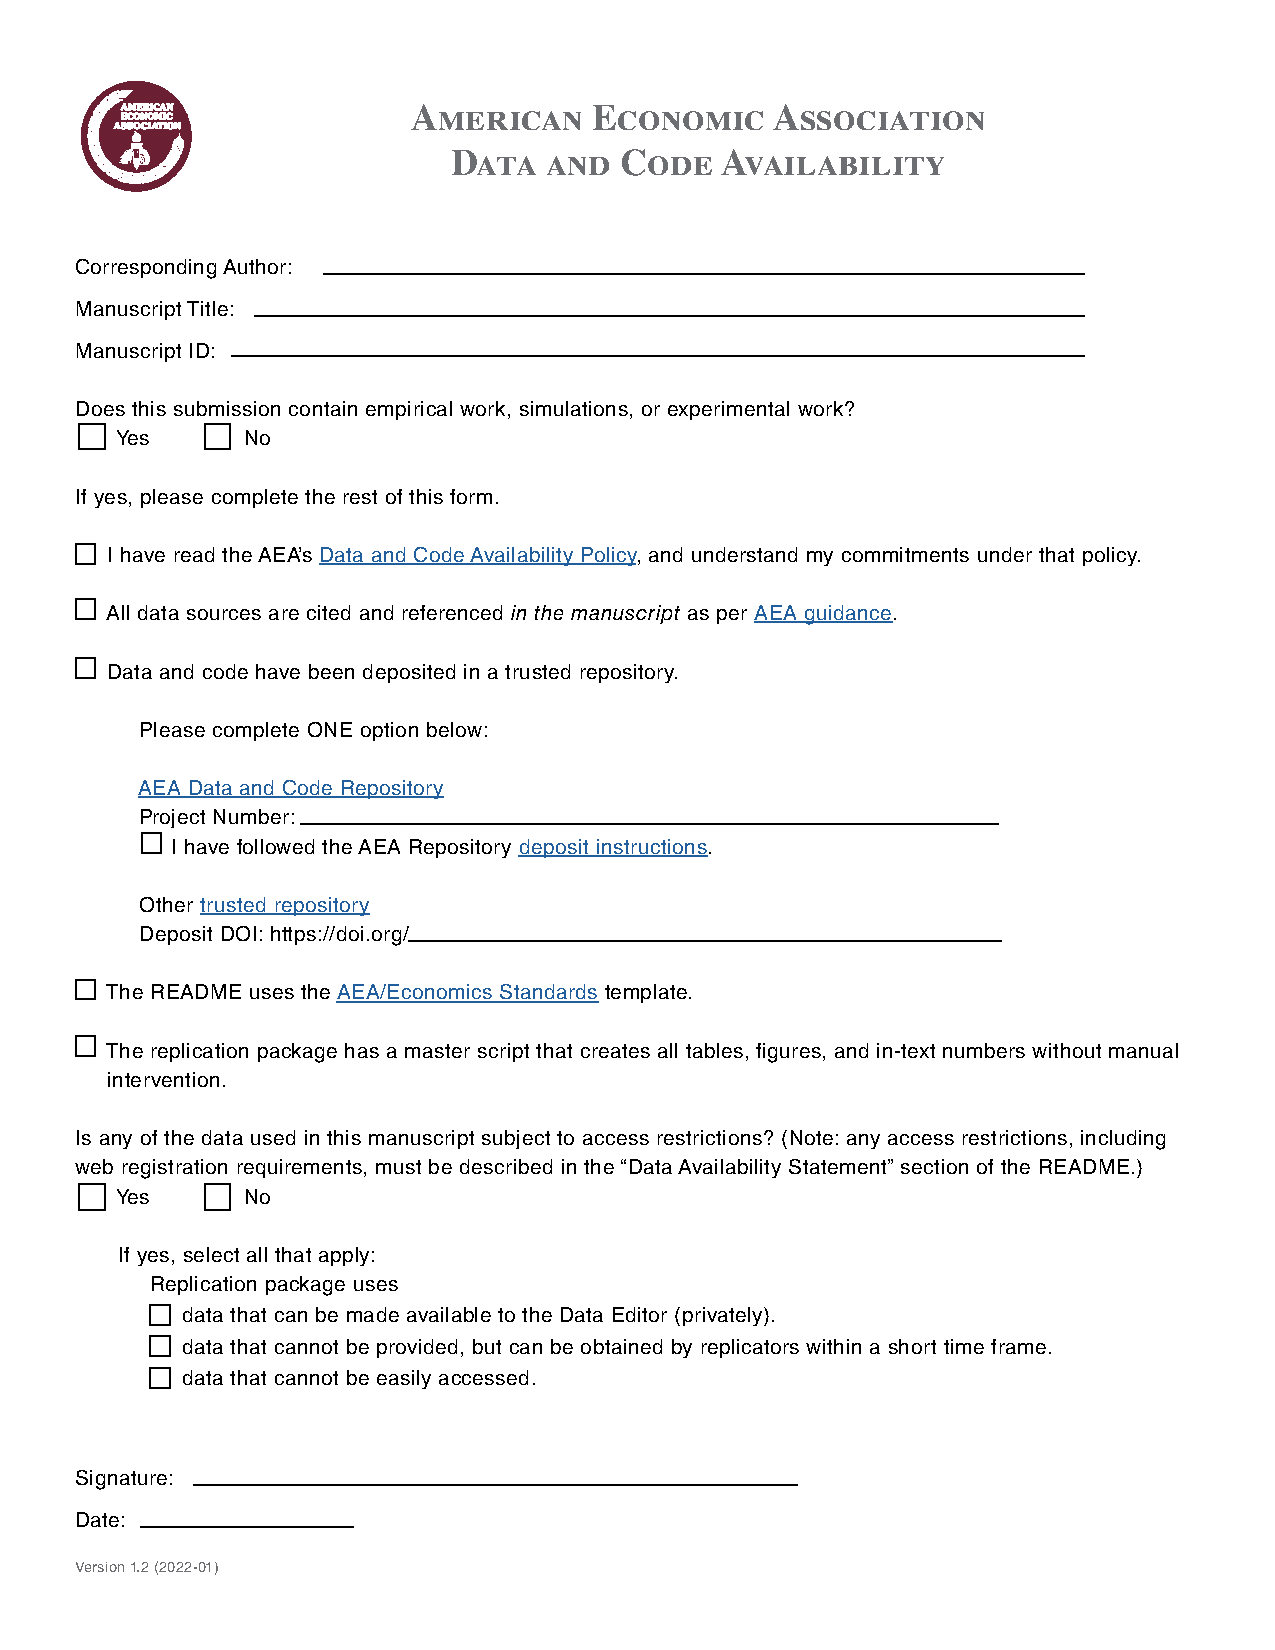
\includepdf[pages=-,pagecommand=\thispagestyle{plain}]{aer_avail.pdf}

\section{Springer Old and New Research Data Policy}
\label{springer}
\subsection{Legacy Data Policy}

\href{https://www.springernature.com/gp/authors/research-data-policy/research-data-policy-types}{Springer Data Policy}

All Springer Nature journals are moving to a policy that requires data availability statements for primary research articles. This is already in place for BMC, Nature and SpringerOpen titles and is being progressively adopted by Springer and Palgrave Macmillan journals.

While the implementation is underway, certain Springer and Palgrave Macmillan journals will retain the older data policy types, as outlined below. The specific data policy of each journal is stated in the submission guidance. ‘Type 3’ is equivalent to our new, standardised data policy.
Our legacy data policies

Policy Type	Policy summary:\\
Type 1: Data sharing and data citation is encouraged\\
Type 2: Data sharing and evidence of data sharing encouraged\\
Type 3: Data sharing encouraged and statements of data availability required\\
Type 4: Data sharing, evidence of data sharing and peer review of data required\\

\subsection{New Research Data Policy}
https://www.springernature.com/gp/authors/research-data-policy

Research data policy

At Springer Nature we advance discovery by publishing trusted research, supporting the development of new ideas and championing open science. We also aim to facilitate compliance with research funder and institution requirements to share data.

To help accomplish this we have established a standard research data policy for our journals, based on transparency around supporting data. This policy applies to all datasets that are necessary to interpret and replicate the conclusions reported in a research article.
\begin{enumerate}
	\item \textbf{All original articles must include a data availability statement.}\\
	
	Data availability statements should include information on what data are available, where these can be found, and any applicable access terms. This applies to both original and reused data, and whether or not data can be shared publicly. See our guidance on data availability statements for more information.
	
	\item \textbf{We strongly encourage that all datasets supporting the analysis and conclusions of the paper are made publicly available at the time of publication, and we mandate the sharing of community-endorsed data types.}\\
	
	We encourage authors to deposit their supporting data in publicly available repositories, or failing this within the manuscript or additional supporting files. See our repository guidance for more information.
	
	For a number of data types, submission to a community-endorsed, public repository is mandatory. See our list of mandated data types.
	
	\item \textbf{Peer reviewers are entitled to request access to underlying data (and code) when needed to perform their evaluation of a manuscript.}\\
	
	\item \textbf{We recognise it is not always possible to share research data publicly, for instance when privacy of research participants could be compromised. In such instances data availability should still be stated in the manuscript along with any conditions for access.}\\
	
	A large number of our journals already support this policy, including Nature Portfolio, BMC and many Springer and Palgrave titles. We are in the process of implementing this policy across the remainder of our portfolio in stages.
\end{enumerate}


\newpage
\bibliographystyle{apalike}
\bibliography{./replic_economica}

\end{document}